%% LyX 2.0.3 created this file.  For more info, see http://www.lyx.org/.
%% Do not edit unless you really know what you are doing.
\documentclass[english]{article}
\usepackage[T1]{fontenc}
\usepackage[latin9]{inputenc}
\usepackage{babel}
\usepackage{graphicx}
\usepackage[unicode=true]
 {hyperref}

\makeatletter
%%%%%%%%%%%%%%%%%%%%%%%%%%%%%% Textclass specific LaTeX commands.
\newenvironment{lyxcode}
{\par\begin{list}{}{
\setlength{\rightmargin}{\leftmargin}
\setlength{\listparindent}{0pt}% needed for AMS classes
\raggedright
\setlength{\itemsep}{0pt}
\setlength{\parsep}{0pt}
\normalfont\ttfamily}%
 \item[]}
{\end{list}}

\makeatother

\begin{document}

\title{Grafika gier 3D od podstaw}

\maketitle
Tr�jwymiarowe gry komputerowe ju\.{z} niemal od dw�ch dekad rz\k{a}dz\k{a}
si\k{e} tymi samymi prawami. Spr�bujemy zbudowa\'{c} minimalistyczny
silnik 3D i zbada\'{c} podstawy jego dzia\l{}ania. 


\section{Wprowadzenie}

Tekst ten ma by\'{c} tak prosty jak tylko to mo\.{z}liwe. Zar�wno
od strony programistycznej jak i matematycznej. W za\l{}o\.{z}eniu
powinien by\'{c} on zrozumia\l{}y dla bystrego dwunastolatka. Przynajmniej
mam tak\k{a} nadziej\k{e}.

W odr�\.{z}nieniu od wi\k{e}kszo\'{s}ci podobnych przewodnik�w, skupimy
si\k{e} na podstawach, poczynaj\k{a}c od pojedy\'{n}czych pikseli
i tr�jk\k{a}t�w. Stworzymy ca\l{}kowicie programowy silnik, bez pomocy
OpenGL czy innych podobnych bibliotek. Ostatecznie b\k{e}dzie on wy\'{s}wietla\l{}
ruchomy model \l{}omu pobrany z pliku zewn\k{e}trznego z dodatkiem
cieniowania p\l{}askiego.

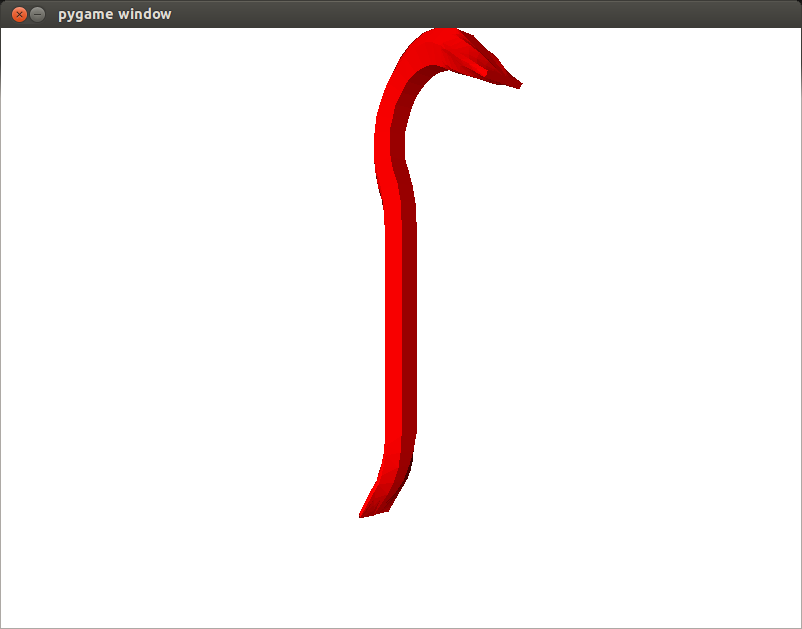
\includegraphics[scale=0.4]{1_crowbar}

Nie b\k{e}dziemy si\k{e} skupia\'{c} na operacjach na macierzach,
tam gdzie nie jest to konieczne jak r�wnie\.{z} nie \textquotedblright{}edziemy
zajmowa\'{c} si\k{e} bardziej wymy\'{s}lnymi rozwi\k{a}zaniami w grafice
3D jak wsp�\l{}rz\k{e}dne jednorodne.

Ca\l{}o\'{s}\'{c} powstanie w j\k{e}zyku skryptowym Python. Wyb�r
wydaje si\k{e} ma\l{}o sensowny dla silnika 3D, z uwagi na bardzo
nisk\k{a} wydajno\'{s}\'{c}, ale przecie\.{z} nie chodzi nam o wydajno\'{s}\'{c}
a o prostot\k{e} i walory edykacyjne. B\k{e}dziemy te\.{z} unika\'{c}
bardziej zaawansowanych element�w programowania jak klasy czy obiekty.
Ca\l{}o\'{s}\'{c} ma by\'{c} zrozumia\l{}a nawet dla ludzi bez do\'{s}wiadczenia
programistycznego, a kod ma si\k{e} zamkn\k{a}\'{c} w oko\l{}o 300
liniach i ma dzia\l{}a\'{c} zar�wno pod Linuksem jak i Windowsem.

Opr�cz \href{http://www.python.org/}{Pythona} (u\.{z}y\l{}em wersji
2.7) wykorzystamy te\.{z} bibliotek\k{e} \href{http://www.pygame.org/news.html}{PyGame},
kt�ra pomo\.{z}e nam wy\l{}\k{a}cznie w rysowaniu okna i wype\l{}nianiu
go pikseli. Python jest ju\.{z} zwykle domy\'{s}lnie zainstalowany
w wi\k{e}kszo\'{s}ci dystrycucji, a PyGame mo\.{z}na znale\'{z}\'{c}
w pakiecie \emph{python-pygame}.

Po otwarciu konsoli i wpisaniu wywo\l{}aniu w niej Pythona, mo\.{z}emy
zacz\k{a}\'{c} eksperymentowa\'{c} widz\k{a}\'{c} na bie\.{z}\k{a}co
wyniki naszych prac:
\begin{lyxcode}
\$~python~~

Python~2.7.4~(default,~Jul~~5~2013,~08:21:57)~~{[}GCC~4.7.3{]}~on~linux2~Type~\textquotedbl{}help\textquotedbl{},~\textquotedbl{}copyright\textquotedbl{},~\textquotedbl{}credits\textquotedbl{}~or~\textquotedbl{}license\textquotedbl{}~for~more~information.~

>\textcompwordmark{}>\textcompwordmark{}>~
\end{lyxcode}
Wychodzimy z interpretera wciskaj\k{a}\'{c} \emph{Ctrl-D}. Mo\.{z}emy
te\.{z} zapisywa\'{c} kod w plika\'{c} tekstowych i wywo\l{}ywa\'{c}
je w nast\k{e}puj\k{a}cy spos�b:
\begin{lyxcode}
\$~python~naszprogram.py
\end{lyxcode}
Na pocz\k{a}tek uruchomimy prosty program wy\'{s}wietlaj\k{a}cy puste
okno - umo\.{z}liwi on sprawdzenie czy PyGame jest prawid\l{}owo zainstalowane.
Utw�rzmy plik z rozszerzeniem {*}.py maj\k{a}cy nast\k{e}puj\k{a}c\k{a}
tre\'{s}\'{c}:
\begin{lyxcode}
import~pygame

def~main():

~~~~xw~=~800

~~~~yw~=~600~~~~~

~~~~screen~=~pygame.display.set\_mode((xw,~yw))

~~~~running~=~True~~~~~~~~~~

~~~~~~~~while~running:~~~~~~~~~

~~~~~~~~for~event~in~pygame.event.get():~\#przerwanie~petli

~~~~~~~~~~~~if~event.type~==~pygame.QUIT:

~~~~~~~~~~~~~~~~running~=~False

main()
\end{lyxcode}
Warto zauwa\.{z}y\'{c}, \.{z}e Python nie wykorzystuje nawias�w do
zamykanie p\k{e}tli (for, while), ani do instrukcji warunkowych (if).
Jest za to wra\.{z}liwy na wci\k{e}cia. Proponuj\k{e} u\.{z}ywa\'{c}
czterech spacji jako wci\k{e}cia. Wiele edytor�w tekstu ma te\.{z}
opcj\k{e} umo\.{z}liwiaj\k{a}c\k{a} automatycz\k{a} konwersj\k{e}
tabulator�w na spacje. Poni\.{z}ej ustawienia w edytorze Gedit.

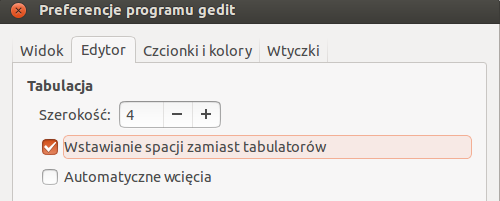
\includegraphics{2_gedit}


\section{Rzutowanie perspektywiczne}

W grach stosowane jest rzutowanie perspektywiczne, odpowiadaj\k{a}ce
rzeczywisto\'{s}ci, gdzie dalsze obiekty wydaj\k{a} si\k{e} mniejsze.
W innych zastosowaniach, np. oprogramowanie CAD, mo\.{z}na spotka\'{c}
te\.{z} rzutowanie r�wnoleg\l{}e, kt�rym nie b\k{e}dziemy si\k{e}
tutaj zajmowa\'{c}.

Wyobra\'{z}my sobie, \.{z}e nie patrzymy na ekran komputera a na obiekt
znajduj\k{a}cy si\k{e} za oknem. Szyba tego okna jest odpowiednikiem
naszego ekranu, kt�rego nazywa\'{c} te\.{z} b\k{e}dziemy p\l{}aszczyzn\k{a}
rzutowania. Za oknem znajduje si\k{e} kartonowe pud\l{}o. Bierzemy
flamaster do r\k{e}ki i zaczynamy zaznacza\'{c} na szybie punkty tak
aby si\k{e} pokrywa\l{}y z wierzcho\l{}kami (naro\.{z}nikami) pud\l{}a.
Potem \l{}\k{a}czymy liniami narysowane punkty i ostatecznie zamalowujemy
obszary zamkni\k{e}te przez te linie. W\l{}a\'{s}nie utworzyli\'{s}my
na szybie rzut perspektywiczny naszego obiektu 3D (pud\l{}a).


\section{Rasterizer tr�jk\k{a}ta}


\section{Transformacje}


\section{Wczytywanie modeli}


\section{Cieniowanie p\l{}askie}
\end{document}
